Muchas de las grandes empresas que conocemos el día de hoy, como Google, Apple, Microsoft, entre otras, desarrollan su propia tecnología para interpretar un texto simple y analizarlo con el objetivo que el computador pueda interpretar el contexto de la oración. Por un lado podemos observar a empresas como Apple INC. que desarrollan un framework llamado 'NSLinguisticTagger' \cite{NSLinguisticTagger}, el gigante de Google desarolla 'Syntaxnet' \cite{SyntaxnetGH}, y muchas empresas suman y aportan más tecnologías. En este caso, analizaremos SyntaxNet puesto que en el 2016 la declararon Open Source. Esto significa que nosotros, los usuarios, podemos utilizar, cambiar y redistribuir el software, a cualquiera, para cualquier propósito, ya sea en su forma modificada o en su forma original \cite{OpenSource}.

Un gran problema al desarrollar este tipo de tecnologías es que el lenguaje que utilizamos nosotros, los seres humanos, tiene grandes niveles de ambigüedad (propiedad muy conocida al analizar las Gramáticas Independientes del Contexto). Google AI \cite{GoogleAISyntaxNet} nos menciona que es muy común encontrarse con oraciones de 20 a 30 palabras que cuenten con miles o cientos de miles posibilidades sintácticas. ¿Esto qué quiere decir? Que el computador tiene que buscar entre esas alternativas y encontrar la estructura más plausible dado el contexto. 

En este caso vamos a mencionar un ejemplo expuesto por Google AI \cite{GoogleAISyntaxNet}. 

\begin{figure}[h!]
    \centering
    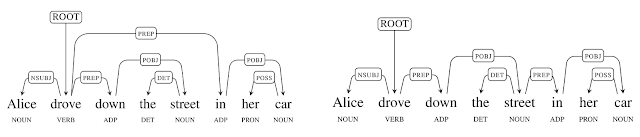
\includegraphics[width=\textwidth]{img/EjemploAmbiguedad.png}
    \caption{Ejemplo de Ambiguedad de Google AI \cite{GoogleAISyntaxNet}}
    \label{fig:AmbEjm}
\end{figure} 

En la siguiente oración: 'Alice drove down the street in her car.' (Alice condujo por la calle en su auto.) podemos obtener 2 interpretaciones: La correcta, señala que Alice está efectivamente manejando su auto, y la segunda nos indica que la calle está ubicada en el carro (posible sintácticamente, pero absurdo). Este es un claro ejemplo de ambigüedad donde el computador tiene que interpretar de manera correcta el contexto de la oración.

Google AI \cite{GoogleAISyntaxNet} también nos menciona que nosotros, como seres humanos, somos expertos en resolver estos problemas de ambigüedad. Somos tan expertos que ni siquiera notamos que estamos procesando esto en nuestro cerebro. El verdadero desafío está en que el computador realice las interpretaciones de manera correcta.

Nosotros sabemos que el problema de la ambigüedad no tiene una solución exacta. Por ello, todos los métodos para resolver la ambigüedad serán métodos de aprendizaje estadísticos, en el sentido de que intentan hacer una generalización inductiva a partir de los datos observados y utilizarlos para hacer inferencias con respecto a datos nunca vistos anteriormente \cite{Amb}. Estos métodos estadísticos, hoy en día, están considerados dentro de la rama de la Inteligencia Artificial. Roth \cite{Amb} nos menciona que existen cuatro aproximaciones para resolver el problema de la desambigüedad: The naive Bayes estimation (Duda ~ Hart 1973), Katz's back-off model, transformation based learning (Brill 1995) y el Decision Lists (Yarowsky 1995).

Todas estas aproximaciones buscan una superficie de decisión que sea una función lineal en el espacio de características. Esto quiere decir que los métodos asumen que el espacio está dividido en una función lineal, con la propiedad de que en una de  las regiones definidas, la predicción más probable es 0 y en la otra, la predicción más probable es 1. \cite{Amb}

Empresas como Google no son ajenas a estas técnicas de AI expuestas. Ellos utilizan estos métodos para resolver los problemas de ambigüedad. En este caso, 'SyntaxNet' utiliza redes neuronales para resolver el problema de la ambigüedad. Pero, ¿cómo lo hacen?. Google AI \cite{GoogleAISyntaxNet} nos señala que procesan una oración de izquierda a derecha en donde cada palabra de la oración es considerada en el algoritmo. Cabe recalcar que llegan a un punto donde encuentran varias soluciones posibles, pero debido a la ambigüedad, no pueden llegar a una decisión prematura. Por esta razón, utilizan un 'Beam search' (optimización del best-first search) para recorrer el grafo generado e ir descartando posibles hipótesis cuando existan varias otras hipótesis 'rankeadas' con un puntaje más alto y estas estén bajo consideración.

¿Que tan preciso es este modelo? Según Google AI \cite{GoogleAISyntaxNet} se ha logrado una precisión al 94\% después de probar el algoritmo con miles de oraciones en el idioma inglés. Asimismo, en un estudio con lingüistas se comprobó que los seres humanos tienen un 96\%-97\% de precisión. Lograr esta precisión es algo extraordinario, todavía no llegamos a la precisión humana pero estamos muy cerca. Con estos resultados esta tecnología puede aplicarse sin problema en diversas áreas.

Este nuevo modelo se encuentra en el siguiente 'paper' \cite{GoogleAISyntaxPaper} publicado por Google el 19 de marzo del 2016.